\documentclass[border=0.5cm]{standalone}

% this is not done yet, takenr from the R library

\usepackage[latin1]{inputenc}
\usepackage{tikz}

%% using the pgf-umlcd package, see https://github.com/xuyuan/pgf-umlcd
\usepackage{pgf-umlcd} 
%\usetikzlibrary{shapes,arrows, positioning, decorations.markings}

\renewcommand{\umlfillcolor}{blue!10}
\renewcommand{\umldrawcolor}{black}

\begin{document}
\pagestyle{empty}


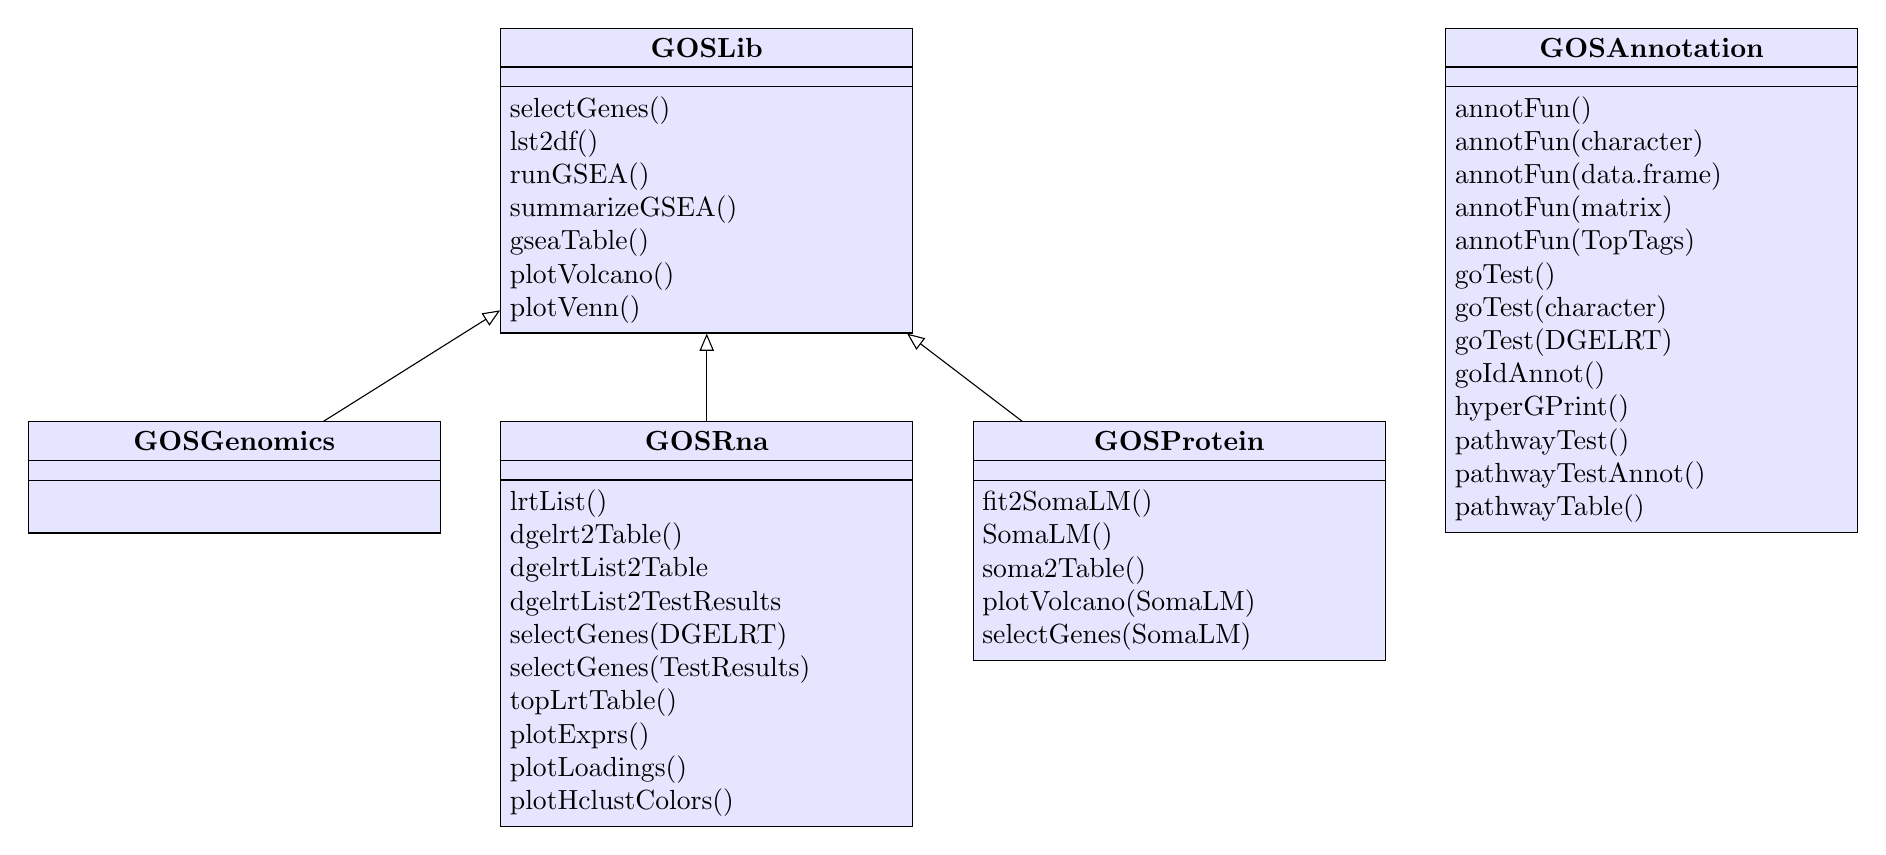
\begin{tikzpicture}

  \begin{class}[text width=5cm]{GOSLib}{0,0}
    %\attribute{owner : String}
    %\attribute{balance : Dollars = 0}
    \operation{selectGenes()}
    \operation{lst2df()}
    \operation{runGSEA()}
    \operation{summarizeGSEA()}
    \operation{gseaTable()}
    \operation{plotVolcano()}
    \operation{plotVenn()}
  \end{class}

  \begin{class}[text width=5cm]{GOSGenomics}{-6,-5}
    \inherit{GOSLib}
    \attribute{}
    \operation{}
    \operation{}
  \end{class}

  \begin{class}[text width=5cm]{GOSRna}{0,-5}
    \inherit{GOSLib}
    \attribute{}
    \operation{lrtList()}
    \operation{dgelrt2Table()}
    \operation{dgelrtList2Table}
    \operation{dgelrtList2TestResults}
    \operation{selectGenes(DGELRT)}
    \operation{selectGenes(TestResults)}
    \operation{topLrtTable()}
    \operation{plotExprs()}
    \operation{plotLoadings()}
    \operation{plotHclustColors()}
  \end{class}

  \begin{class}[text width=5cm]{GOSProtein}{6,-5}
    \inherit{GOSLib}
    \attribute{}
    \operation{fit2SomaLM()}
    \operation{SomaLM()}
    \operation{soma2Table()}
    \operation{plotVolcano(SomaLM)}
    \operation{selectGenes(SomaLM)}
  \end{class}


  \begin{class}[text width=5cm]{GOSAnnotation}{12,0}
    %\attribute{owner : String}
    %\attribute{balance : Dollars = 0}
    \operation{annotFun()}
    \operation{annotFun(character)}
    \operation{annotFun(data.frame)}
    \operation{annotFun(matrix)}
    \operation{annotFun(TopTags)}
    \operation{goTest()}
    \operation{goTest(character)}
    \operation{goTest(DGELRT)}
    \operation{goIdAnnot()}
    \operation{hyperGPrint()}
    \operation{pathwayTest()}
    \operation{pathwayTestAnnot()}
    \operation{pathwayTable()}
  \end{class}

\end{tikzpicture}

\end{document}

%%% Local Variables:
%%% mode: latex
%%% TeX-master: t
%%% End:
